% ═══════════════════════════════════════════════════════════════════════
\section{La distance de Hausdorff}
% ═══════════════════════════════════════════════════════════════════════

\begin{frame}{Une distance entre des ensembles}
  \small Notons $\Comp{E}$ l'ensemble des sous-ensembles compacts
  non vides d'un espace métrique $(E,d)$.
  \vspace{6pt}

  L'idée à formaliser : deux ensembles sont proches lorsque
  chaque point de l'un est près d'un point de l'autre, et
  réciproquement.
  \vspace{6pt}

  Outil : le voisinage d'un ensemble, obtenu en l'« épaississant ».
  \vspace{6pt}

  Objectif lointain : au chapitre 3, une figure fractale sera
  un point de l'espace métrique $\big(\Comp{\R^2},\dH\big)$.
\end{frame}

\subsection[Le epsilon-voisinage et la somme de Minkowski]{Le \texorpdfstring{$\varepsilon$}{epsilon}-voisinage et la somme de Minkowski}

\begin{frame}{Définitions 2.7 et 2.8 --- Minkowski, $\varepsilon$-voisinage}
  \begin{Enonce}{Définition 2.7 --- Somme de Minkowski}
    \small Soit $(E,d)=(\R^n,\dE)$ et $A,B\subseteq E$. La \defi{somme de
    Minkowski} de $A$ et $B$ est
    $A\oplus B = \{a+b : a\in A,\ b\in B\}$.
  \end{Enonce}
  \small Une copie de $B$ placée en chaque point de $A$, puis on réunit
  tout. Si $B$ est une petite boule fermée centrée à l'origine : on
  ajoute autour de $A$ une bande de même épaisseur dans toutes les
  directions.
  \begin{Enonce}{Définition 2.8 --- $\varepsilon$-voisinage d'un ensemble}
    \small Soit $A\subseteq\R^n$ non vide et $\varepsilon>0$. Le
    \defi{$\varepsilon$-voisinage} de $A$ est
    $\Vois{A}{\varepsilon} = A\oplus\overline{\boule{0}{\varepsilon}}$,
    où $\overline{\boule{0}{\varepsilon}} = \{x : \dE(x,0)\leq\varepsilon\}$
    est la boule fermée.
  \end{Enonce}
\end{frame}

\begin{frame}{Figure 2.8 --- Le $\varepsilon$-voisinage}
  \begin{columns}[c]
    \begin{column}{0.5\textwidth}
      \small Reformulation :
      \[
        \begin{aligned}
          \Vois{A}{\varepsilon} = \{x\in E :\ & \dE(x,a)\leq\varepsilon\\
          & \text{pour un certain } a\in A\},
        \end{aligned}
      \]
      les points à distance au plus $\varepsilon$ d'au moins un
      point de $A$.
      \vspace{6pt}

      En particulier $A\subseteq\Vois{A}{\varepsilon}$ : chaque point
      de $A$ est à distance $0\leq\varepsilon$ de lui-même.
    \end{column}
    \begin{column}{0.48\textwidth}
      \FigBox[0.55\textheight]{%
        \begin{tikzpicture}[scale=0.9]
          \draw[sectioncolor, thick, fill=steelblue4!28] plot[smooth cycle, tension=0.75]
            coordinates {(-0.49,-0.20) (0.99,-1.01) (2.75,-0.47) (3.16,1.02)
                         (1.81,2.23) (0.19,1.83)};
          \draw[fig] plot[smooth cycle, tension=0.75]
            coordinates {(0,0) (1.1,-0.6) (2.4,-0.2) (2.7,0.9) (1.7,1.8) (0.5,1.5)};
          \node[etiq, sectioncolor] at (1.2,0.6) {$A$};
          \node[etiq, sectioncolor] at (2.7,2.35) {$\Vois{A}{\varepsilon}$};
          \draw[fleche, sectioncolor] (1.85,1.55) -- (2.5,2.05);
          \draw[sectioncolor, thick, {Stealth[length=2mm]}-{Stealth[length=2mm]}]
            (2.1,-0.3) -- (2.8,-0.3);
          \node[etiq, sectioncolor, below] at (2.45,-0.35) {$\varepsilon$};
        \end{tikzpicture}}
      \scriptsize (Dessin simplifié : une homothétie plutôt que la vraie
      somme de Minkowski.)
    \end{column}
  \end{columns}
\end{frame}

\begin{frame}{Remarque 2.5 --- Le voisinage dépend aussi de la métrique}
  \begin{Rem}{Remarque 2.5}
    Comme les boules (figure 2.5), le $\varepsilon$-voisinage change
    d'aspect avec la métrique. Pour le singleton $A=\{(0,0)\}$ :
    \begin{itemize}
      \item avec une boule fermée de $(\R^2,\dE)$ : un disque
        plein de rayon $\varepsilon$ ;
      \item avec une boule fermée de $(\R^2,\dT)$ : un carré
        plein tourné de $45^\circ$, de « demi-diagonale » $\varepsilon$.
    \end{itemize}
  \end{Rem}
\end{frame}

\subsection{Définition de la distance de Hausdorff}

\begin{frame}{Définition 2.9 --- Distance de Hausdorff}
  \begin{Enonce}{Définition 2.9 --- Distance de Hausdorff}
    Soit $(E,d)=(\R^n,\dE)$ et $A,B\in\Comp{E}$. La \defi{distance de
    Hausdorff} entre $A$ et $B$ est
    \[
      \dH(A,B) = \inf\{\varepsilon>0 : A\subseteq\Vois{B}{\varepsilon}
      \text{ et } B\subseteq\Vois{A}{\varepsilon}\}.
    \]
  \end{Enonce}
  \small Le plus petit rayon d'épaississement tel que chacun des
  deux ensembles soit recouvert par le $\varepsilon$-voisinage de
  l'autre.
  \begin{itemize}
    \item $A$, $B$ compacts donc bornés : un tel $\varepsilon$ existe
      toujours (assez grand).
    \item On peut montrer que l'infimum est en fait atteint.
  \end{itemize}
\end{frame}

\begin{frame}{Figure 2.9 --- La formule de calcul}
  \begin{columns}[c]
    \begin{column}{0.5\textwidth}
      \small Avec $d(x,C) = \inf_{c\in C} d(x,c)$ :
      \[
        \dH(A,B) = \max\Big\{\sup_{a\in A} d(a,B),\ \sup_{b\in B} d(b,A)\Big\}.
        \tag{2.1}
      \]
      Recette : trouver le point de $A$ le plus loin de $B$ ;
      puis le point de $B$ le plus loin de $A$ ; garder la plus grande
      des deux distances.
    \end{column}
    \begin{column}{0.48\textwidth}
      \FigBox[0.55\textheight]{%
        \begin{tikzpicture}[scale=1.15]
          \draw[firebrick3, thick, fill=firebrick3, fill opacity=0.3] (0,0) circle (1.3);
          \node[etiq, firebrick3] at (-0.75,0.95) {$B$};
          \draw[sectioncolor, thick, fill=steelblue4, fill opacity=0.3,
                rotate around={10:(1.8,0.2)}] (1.8,0.2) ellipse (1.6 and 0.85);
          \node[etiq, sectioncolor] at (2.55,1.15) {$A$};
          \node[pt, label={[etiq]above right:$a^\star$}] (astar) at (3.38,0.48) {};
          \node[ptim, label={[etiq]left:$b^\star$}] (bstar) at (-1.3,0) {};
          \draw[sectioncolor!70, thick, dashed, {Stealth[length=2mm]}-{Stealth[length=2mm]}]
            (astar) -- node[midway, below, etiq]{$d(a^\star,B)$} (1.29,0.18);
          \draw[firebrick3!70, thick, dashed, {Stealth[length=2mm]}-{Stealth[length=2mm]}]
            (bstar) -- node[midway, above, etiq]{$d(b^\star,A)$} (0.22,-0.08);
        \end{tikzpicture}}
    \end{column}
  \end{columns}
\end{frame}

\begin{frame}{Exemple 2.4 --- Deux carrés emboîtés}
  \begin{columns}[c]
    \begin{column}{0.58\textwidth}
      \small $A=\intff{0}{2}\times\intff{0}{2}$,
      $B=\intff{0}{3}\times\intff{0}{3}$.
      \begin{itemize}
        \item $A\subseteq B$ : tout point de $A$ est à distance $0$ de
          $B$, donc $\sup_{a\in A}d(a,B)=0$.
        \item Le point de $B$ le plus loin de $A$ : le coin $(3,3)$, à
          distance $\dE\big((3,3),(2,2)\big)=\sqrt2$.
      \end{itemize}
      \[
        \dH(A,B) = \max\{0,\sqrt2\} = \sqrt2.
      \]
      \scriptsize La formule (2.1) n'est pas symétrique terme à
      terme : c'est le $\max$ qui rend $\dH$ symétrique.
    \end{column}
    \begin{column}{0.4\textwidth}
      \FigBox[0.55\textheight]{%
        \begin{tikzpicture}[scale=0.9]
          \repere{-0.4}{3.4}{-0.4}{3.4}
          \fill[figim] (0,0) rectangle (3,3);
          \fill[fig] (0,0) rectangle (2,2);
          \node[etiq, sectioncolor] at (1,1) {$A$};
          \node[etiq, firebrick3] at (2.6,0.6) {$B$};
          \node[ptim, label={[etiq]above right:$(3,3)$}] (p) at (3,3) {};
          \node[pt] (q) at (2,2) {};
          \draw[firebrick3, thick, dashed] (q) -- node[etiq, above left]{$\sqrt2$} (p);
        \end{tikzpicture}}
    \end{column}
  \end{columns}
\end{frame}

\begin{frame}{Remarque 2.6 --- Pourquoi des ensembles compacts ?}
  \begin{Rem}{Remarque 2.6}
    \small La restriction aux compacts sert à garantir la
    séparation (axiome (b)).
    \vspace{4pt}

    Contre-exemple sans compacité : dans $(\R,\dE)$,
    $A=\intoo{0}{1}$ et $B=\intff{0}{1}$ sont distincts, et pourtant
    $\dH(A,B)=0$ : tout point de $B$ est aussi près qu'on veut d'un
    point de $A$. Le coupable : $A$ n'est pas fermé, il lui « manque »
    ses points frontières.
    \vspace{4pt}

    Sur $\Comp{E}$, on démontre que $\dH(A,B)=0 \Rightarrow A=B$ ; on
    vérifie aussi symétrie et inégalité triangulaire.
  \end{Rem}
  \vspace{4pt}
  \begin{center}
    $(\Comp{E},\dH)$ est un espace métrique dont les « points »
    sont des ensembles.
  \end{center}
\end{frame}

\begin{frame}{Pour la classe 2.1 --- Comparer deux figures géométriques}
  \begin{Classe}{Comparer deux figures géométriques}
    \small « À quel point ce triangle ressemble-t-il à celui-là ? » La
    distance de Hausdorff rend la question précise :
    \begin{itemize}
      \item deux polygones de forme presque identique, dont un sommet a
        légèrement bougé : petite distance de Hausdorff ;
      \item des figures plus différentes : distance plus grande.
    \end{itemize}
    \vspace{2pt}
    C'est le principe de certains logiciels de reconnaissance de
    formes : un contour détecté dans une image ressemble-t-il
    suffisamment à un contour de référence ?
  \end{Classe}
\end{frame}

\begin{frame}{Note historique 2.2 --- Felix Hausdorff (1868--1942)}
  \footnotesize
  \begin{columns}[T]
    \begin{column}{0.25\textwidth}
      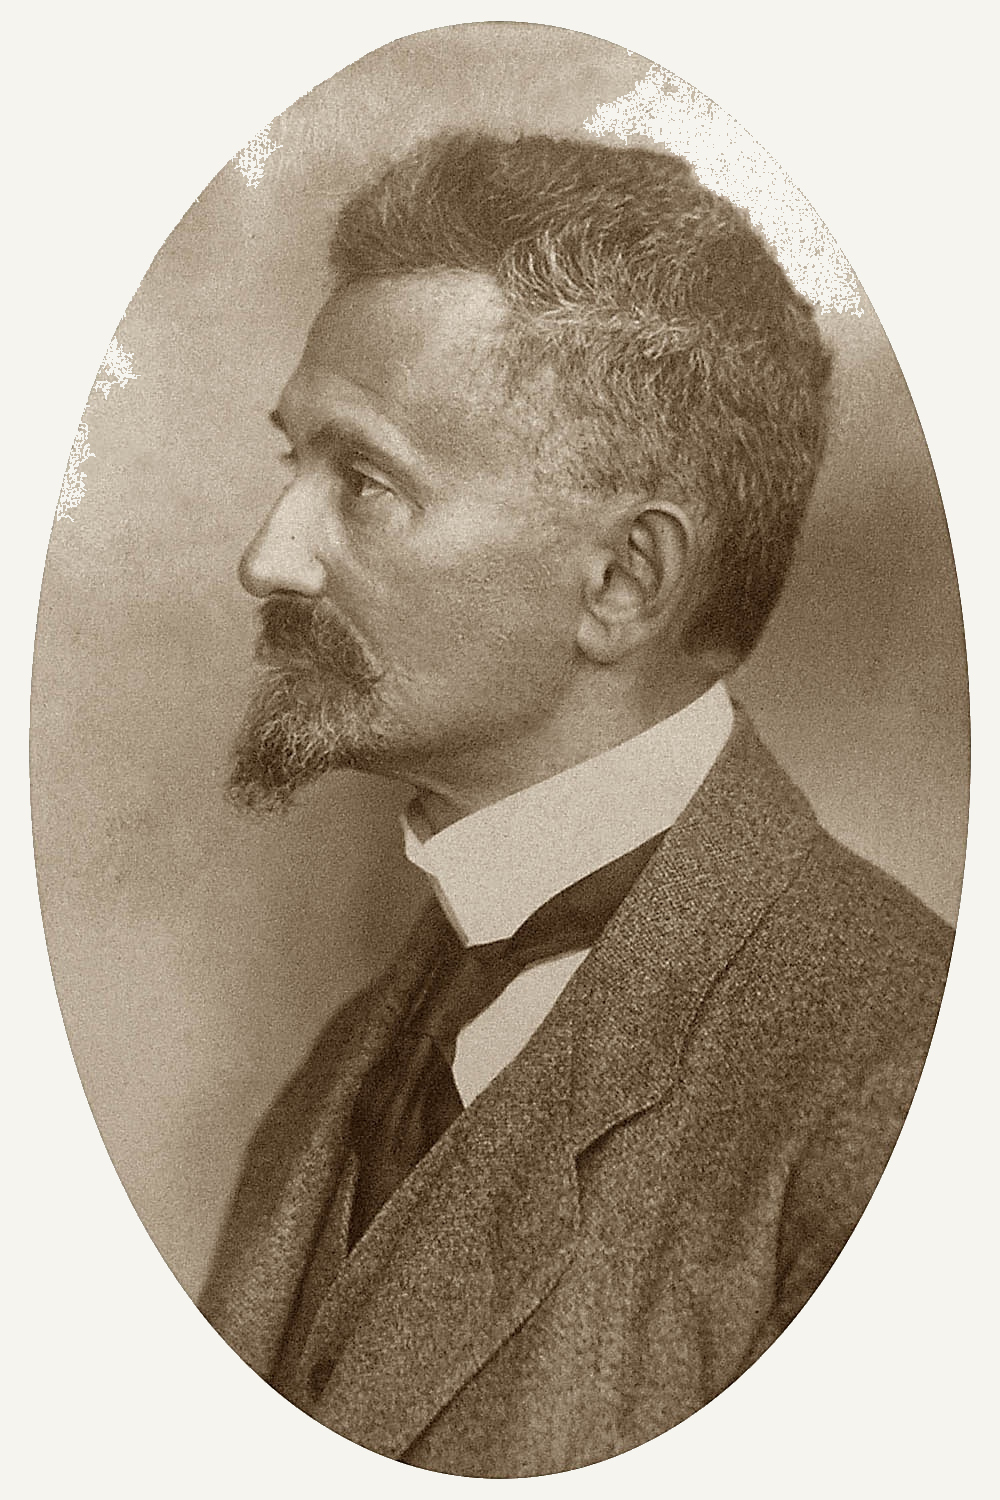
\includegraphics[width=\linewidth]{felix-hausdorff.jpg}\\
      {\scriptsize\color{gray}Felix Hausdorff (1868--1942).
      Domaine public, Wikimedia Commons.}
    \end{column}
    \begin{column}{0.72\textwidth}
      \begin{itemize}
        \item Mathématicien allemand, professeur à Leipzig, Bonn et
          Greifswald.
        \item Grundzüge der Mengenlehre (1914) : les bases de la
          topologie générale telle qu'on l'enseigne encore ;
          c'est là qu'apparaît la distance qui porte son nom.
        \item Aussi poète, essayiste (sur Nietzsche) et dramaturge, sous
          le pseudonyme Paul Mongré.
      \end{itemize}
    \end{column}
  \end{columns}
\end{frame}

\begin{frame}{Note historique 2.2 (suite)}
  \small
  \begin{itemize}
    \item À partir de 1933, persécuté par le régime nazi en raison de
      ses origines juives ; mis à la retraite forcée en 1935 « sans un
      mot de remerciement ».
    \item Après la Nuit de Cristal (1938), ses conditions se
      détériorent encore ; une tentative d'émigration vers les
      États-Unis échoue en 1939.
    \item En janvier 1942, recevant l'ordre de se présenter à un camp
      d'internement, il se donne la mort avec son épouse Charlotte et
      la sœur de celle-ci. Il avait 73 ans.
  \end{itemize}
  \vspace{4pt}
  Une partie de son œuvre, dont la dimension de Hausdorff ---
  outil essentiel de la géométrie des fractales (chapitre 3) --- n'a été
  pleinement reconnue qu'après sa mort.
\end{frame}
